\documentclass{article}

\usepackage[a4paper, margin=1in]{geometry}
\usepackage[onehalfspacing]{setspace} % Correct 1.5 line spacing

\usepackage{graphicx}  % Figures
\graphicspath{{./figures/}}

\usepackage{url}
\usepackage[pdfusetitle]{hyperref}
\usepackage{titlesec}      % Modify title/section/chapter commands
\usepackage{mathtools}     % Various maths related commands
\usepackage{gensymb}       % \degree symbol
\usepackage[thinc]{esdiff} % Derivatives
\usepackage{booktabs}      % \toprule, etc., in tables
\usepackage{doi}           % support DOI links in bibliography
\usepackage{wrapfig}       % figures in text

\usepackage{fontspec}      % Fonts
\usepackage{helvet}
\usepackage{newpxtext,newpxmath}
\defaultfontfeatures{Scale=MatchLowercase, Ligatures=TeX}

\usepackage{algorithm}
\usepackage{algpseudocode}

% SI units
\usepackage{siunitx}
\sisetup{separate-uncertainty=true,number-mode=text,detect-weight=true}
\DeclareSIUnit\belm{Bm}
\DeclareSIUnit\belw{BW}
\DeclareSIUnit\beli{Bi}
\DeclareSIUnit\belz{BZ}

% https://tex.stackexchange.com/a/43009
\DeclarePairedDelimiter\abs{\lvert}{\rvert}%
\DeclarePairedDelimiter\norm{\lVert}{\rVert}%

% Caption figures
\usepackage{caption}
\DeclareCaptionFont{captionlabelfont}{\bfseries \sffamily}
\DeclareCaptionFont{captiontextfont}{\sffamily}
\captionsetup{labelfont=captionlabelfont, textfont=captiontextfont}

% Change footnote style
\renewcommand{\thefootnote}{\fnsymbol{footnote}}

% Fancy header/footer
\usepackage{fancyhdr}
\pagestyle{fancy}
\renewcommand{\sectionmark}[1]{\markright{\thesection . #1}}
\fancyhf{}
\lhead{\fancyplain{}{\thepage}}
\rhead{\fancyplain{}{\textit{\rightmark}}}

% Bibliography
\usepackage[backend=biber, style=ieee, natbib=true,
			url=false, isbn=true, doi=true,
			eprint=false, urldate=long]{biblatex}
%\addbibresource{references-old.bib}
\addbibresource{references.bib}

% biblatex IEEE style leaves empty parentheses when there is no date/year field.
% Since there are no date fields for many online resources, we use
%   https://tex.stackexchange.com/a/151264
% to stop these parentheses from being generated if there is no date field.
\usepackage{xpatch}
\xpatchbibdriver{online}
{\printtext[parens]{\usebibmacro{date}}}
{\iffieldundef{year}
	{}
	{\printtext[parens]{\usebibmacro{date}}}}
{}
{\typeout{There was an error patching biblatex-ieee (specifically, ieee.bbx's @online driver)}}

\renewcommand{\descriptionlabel}[1]{\hspace*{\labelsep}\spacedlowsmallcaps{#1}}

\titlespacing*{\chapter}{0pt}{1\baselineskip}{1.2\baselineskip}
\titlespacing*{\section}{0pt}{1.25\baselineskip}{1\baselineskip} 
\titlespacing*{\subsection}{0pt}{1.25\baselineskip}{1\baselineskip}
\titlespacing*{\paragraph}{0pt}{1\baselineskip}{1\baselineskip}

% Fix for missing µ in siunitx ???
% https://tex.stackexchange.com/a/428215
\sisetup{math-micro=\text{µ},text-micro=µ}

\newcommand\mytitle    {Millimetre-Wave Cloud Profiling Radar}
\newcommand\mysubtitle {Project Report}
\newcommand\myauthor   {180014855}
\newcommand\mydate     {\today}
\newcommand\mymodule   {PH4111}
\newcommand\mywordcount{2300}

\title {\mytitle}
\author{\myauthor}
\date  {\mydate}

%\usepackage[acronym,nonumberlist]{glossaries}
%\usepackage[acronym,nonumberlist]{glossaries-extra}

\usepackage[nopostdot, toc, nogroupskip, nomain, indexonlyfirst, acronym, symbols, style=long4col, stylemods={longextra}, nonumberlist, automake]{glossaries-extra}

\makeglossaries

%\setabbreviationstyle[acronym]{long-short}

\newacronym{ac:daq}{DAQ}{Data acquisition}
\newacronym{ac:simd}{SIMD}{Single instruction, multiple data}
\newacronym{ac:cpr}{CPR}{Cloud profiling radar}
\newacronym{ac:fmcw}{FMCW}{Frequency-modulated continuous wave}
\newacronym{ac:netcdf}{NetCDF}{Network common data form}
\newacronym{ac:openmp}{OpenMP}{Open multi-processing}
\newacronym{ac:adc}{ADC}{Analogue to digital converter}
\newacronym{ac:dds}{DDS}{Direct digital synthesiser}
\newacronym{ac:dft}{DFT}{Discrete Fourier transform}
\newacronym{ac:fftw}{FFTW}{Fastest Fourier Transform in the West}
\newacronym{ac:mkl}{Intel MKL}{Intel Math Kernel Library}
\newacronym{ac:snr}{SNR}{Signal-to-noise ratio}
\newacronym{ac:if}{IF}{Intermediate frequency}
\newacronym{ac:cpi}{CPI}{Coherent processing interval}
\newacronym{ac:cpu}{CPU}{Central processing unit}
\newacronym{ac:cvi}{CVI}{C for Virtual Instrumentation, an ANSI C environment designed by National Instruments.}
\newacronym{ac:fft}{FFT}{Fast Fourier transform}
\newacronym{ac:vla}{VLA}{Variable length array}

\newglossaryentry{gl:fast-time}
{
	name={fast time},
	description={On the time scale of one chirp}
}

\newglossaryentry{gl:slow-time}
{
	name={slow time},
	description={On the time scale of multiple chirps}
}

\glsaddall

\begin{document}

\begin{titlepage}
	\centering
	{
\includegraphics[width=0.3\textwidth]{uos-logo}}
	\par
	{\LARGE\bfseries University of St Andrews\par}
	{\LARGE School of Physics and Astronomy\par}
	\vspace{1.5cm}
	{\huge\bfseries\mytitle\par}
	{\Large\mysubtitle\par}
	\vspace{2cm}
	{\Large\myauthor\par}
	{\large\textbf{Module:} \mymodule\par}
	{\large\textbf{Word count:} \mywordcount\par}
	\vfill
	{\large\today\par}
\end{titlepage}

\begin{abstract}
	Insert abstract here.
\end{abstract}

\tableofcontents
\clearpage
\printglossary

\section{Introduction}

\footnote{The code is available on GitHub.\supercite{Code}}

\section{Signal processing theory}
\subsection{FMCW-Doppler radar}
\acrshort{ac:fmcw} radar emit consecutive chirps - signals whose frequency is linearly modulated by sawtooth waves. The reflected chirp arrives at a time \(\Delta t\) after emission, leading to a phase difference as illustrated in Fig. \ref{fig:Chirp}. The transmitted and received signals are mixed (Fig. \ref{fig:RadarDiagram}) and their intermediate frequency (\acrshort{ac:if}, essentially the difference frequency) is extracted. The target range relates to the time delay and hence the intermediate frequency \(f_{IF}\) by
\begin{equation}
	r = \frac{c \Delta t}{2} = \frac{c f_{IF} T_c}{2 B},
\end{equation}
where \(r\) is the distance from the radar and \(T_c\) is the chirp duration.\supercite{TIFMCWDoppler}
In practice, there are many received signals, thus one performs a discrete Fourier transform of the \acrshort{ac:if} signal to obtain a range profile, known as a range-\acrshort{ac:fft} or \textit{fast time} \acrshort{ac:fft} because of the short timescale (and high sampling rate) over which samples are taken.

\begin{figure}
	\centering
	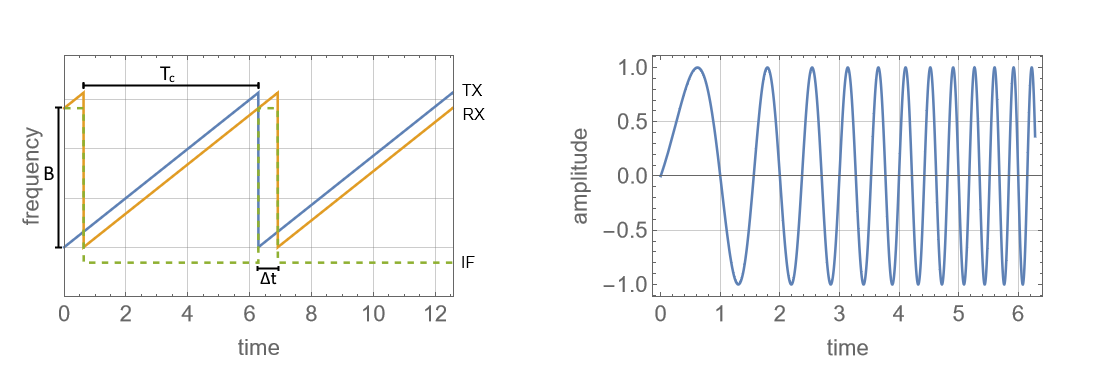
\includegraphics[width=\textwidth]{chirp}
	\caption{Left: transmitted (TX) and received (RX) sawtooth chirps and their difference frequency (IF). Right: illustration of TX chirp waveform. (Own work)}
	\label{fig:Chirp}
\end{figure}

\begin{figure}
	\centering
	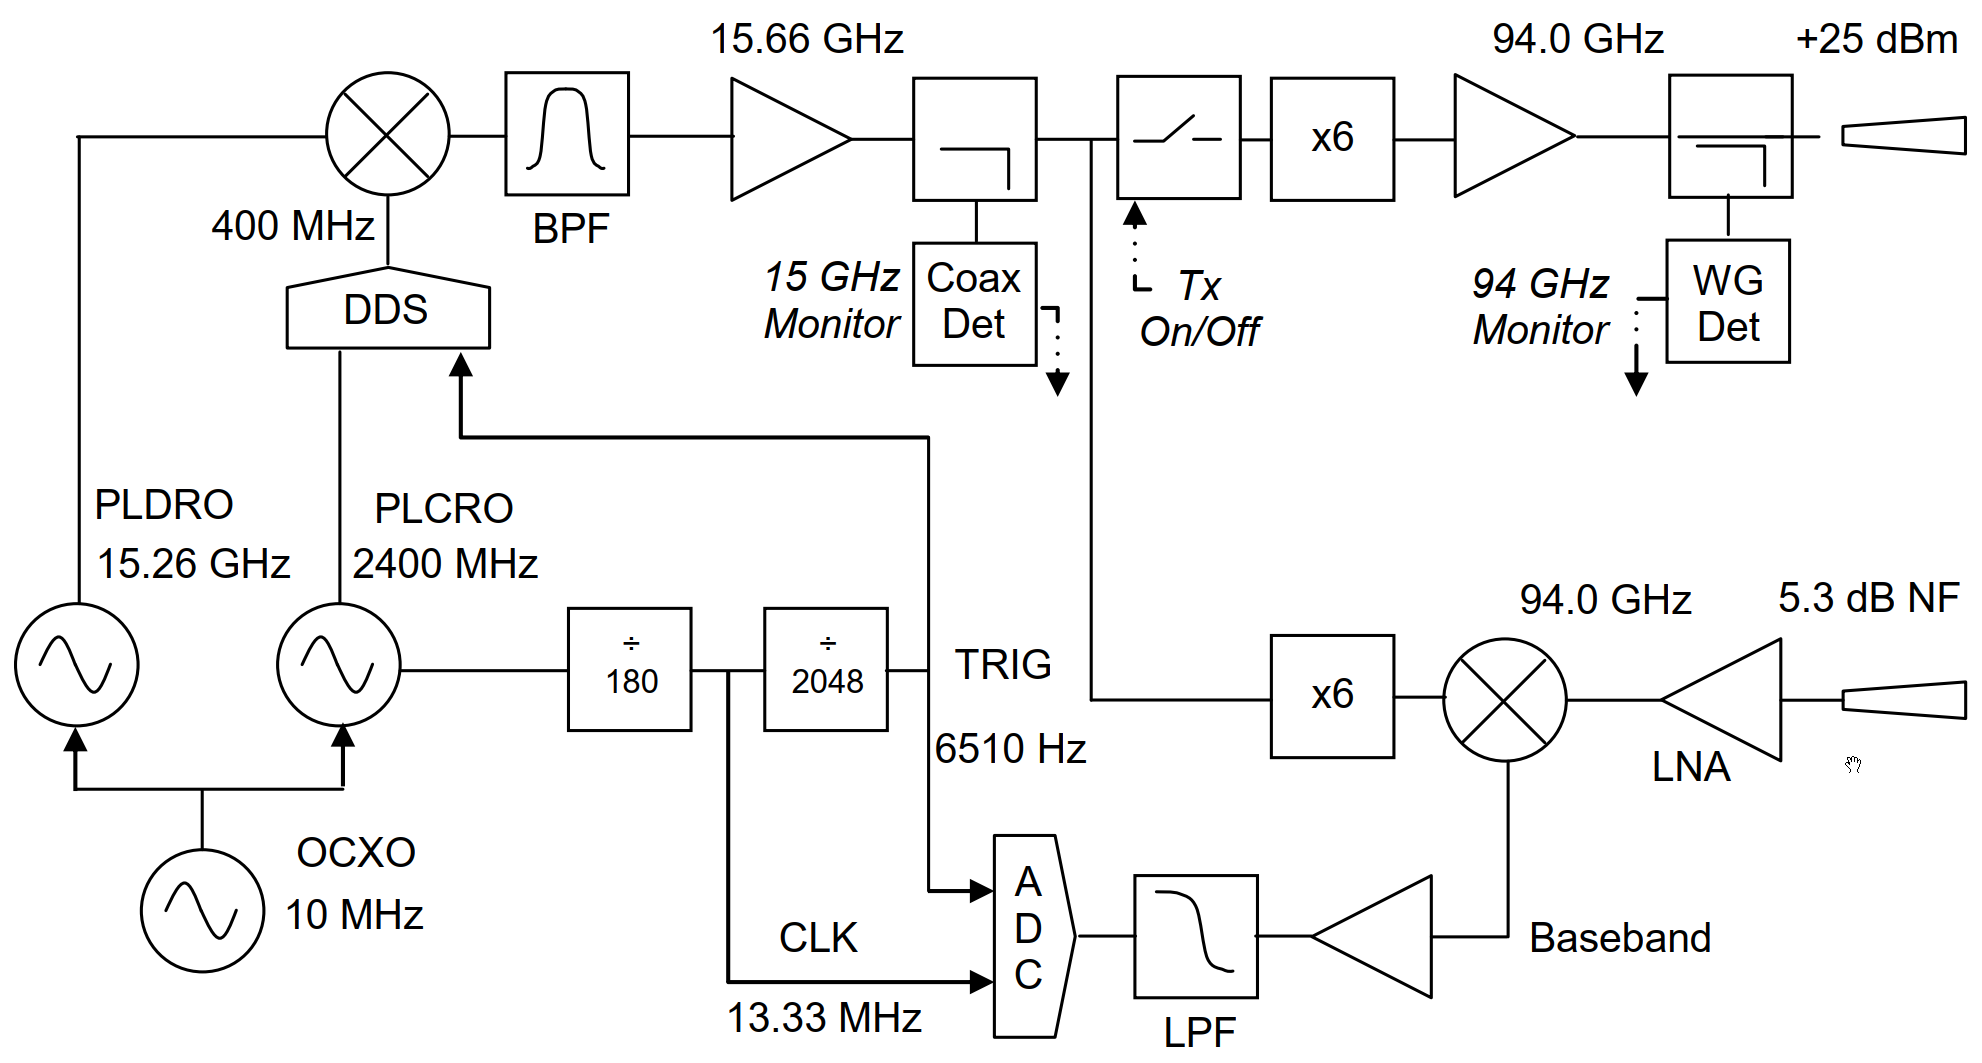
\includegraphics[width=\textwidth]{radar-diagram}
	\caption{Simplified radar system diagram.\supercite{Radar}}
	\label{fig:RadarDiagram}
\end{figure}

To obtain velocity information one extracts the phase change in each range bin across multiple consecutive chirps by performing a Doppler-\acrshort{ac:fft} or \textit{slow time} \acrshort{ac:fft}.
The phase difference \(\delta\) relates to the target velocity \(v\) by\supercite{TIFMCWDoppler}
\begin{equation}
	\delta = \frac{4 \pi v T_c}{\lambda}.
\end{equation}

The sequence of chirps is known as a coherent processing interval (\acrshort{ac:cpi}), the duration of which determines the velocity resolution \(v_{res}\) by
\begin{equation}
	v_{res} = \frac{\lambda}{2 T_f},
\end{equation}
where \(T_f\) is the \acrshort{ac:cpi} duration.

Each \acrshort{ac:cpi} can be thought of as a matrix where each row represents the fast-time samples. The fast-time \acrshort{ac:fft}s are performed row-by-row to get several range profiles and, afterwards, the slow-time \acrshort{ac:fft}s are performed column-by-column to obtain the velocity spectra.

\subsection{Signal averaging}
Explain with signal averaging we can get \(\sqrt{N}\) improvement in SNR, why that's necessary to detect clouds

\begin{figure}
	\centering
	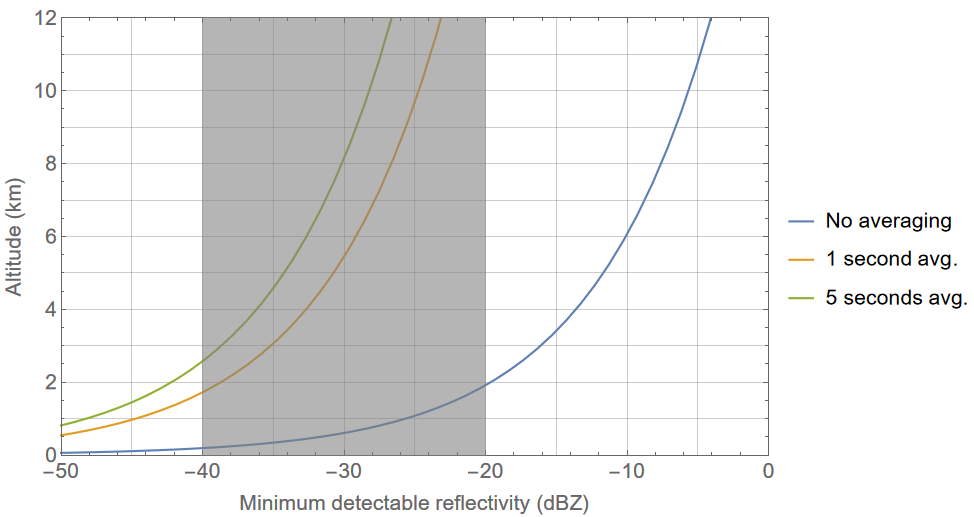
\includegraphics[width=0.6\textwidth]{sensitivity}
	\caption{Radar sensitivity (Own work).}
	\label{fig:Sensitivity}
\end{figure}

\subsection{Doppler moments}
Statistical properties of the velocity spectrum are of great interest to meteorologists. In particular, the mean, variance, skew, and kurtosis ...

\section{Requirements}
There are two software implementations to date, named Mark I and Mark II.
Mark I 

Mark II supports real-time data acquisition (see Sec. \ref{sc:AltToDblBuf}) and saving of raw data (\acrshort{ac:adc} integers) to disk, however does not perform any processing beyond a range-Doppler plot for each \acrshort{ac:cpi}. 

\subsection{User interface and hardware control}
It should also be noted that these implementations exclusively deal with the data acquisition and processing aspect of radar software. The hardware control runs in a separate process. One of the extra project goals is to add a hardware control panel containing controls for bandwidth, chirp or continuous wave mode, transmitter on/off as well as output from various sensors. The panel could be switched between engineering and operational mode, where operational mode hides low-level controls and replaces them with more intuitive controls, such as range resolution instead of bandwidth. The panel would also contain controls for adjusting averaging time and velocity resolution.

\begin{figure}
	\centering
	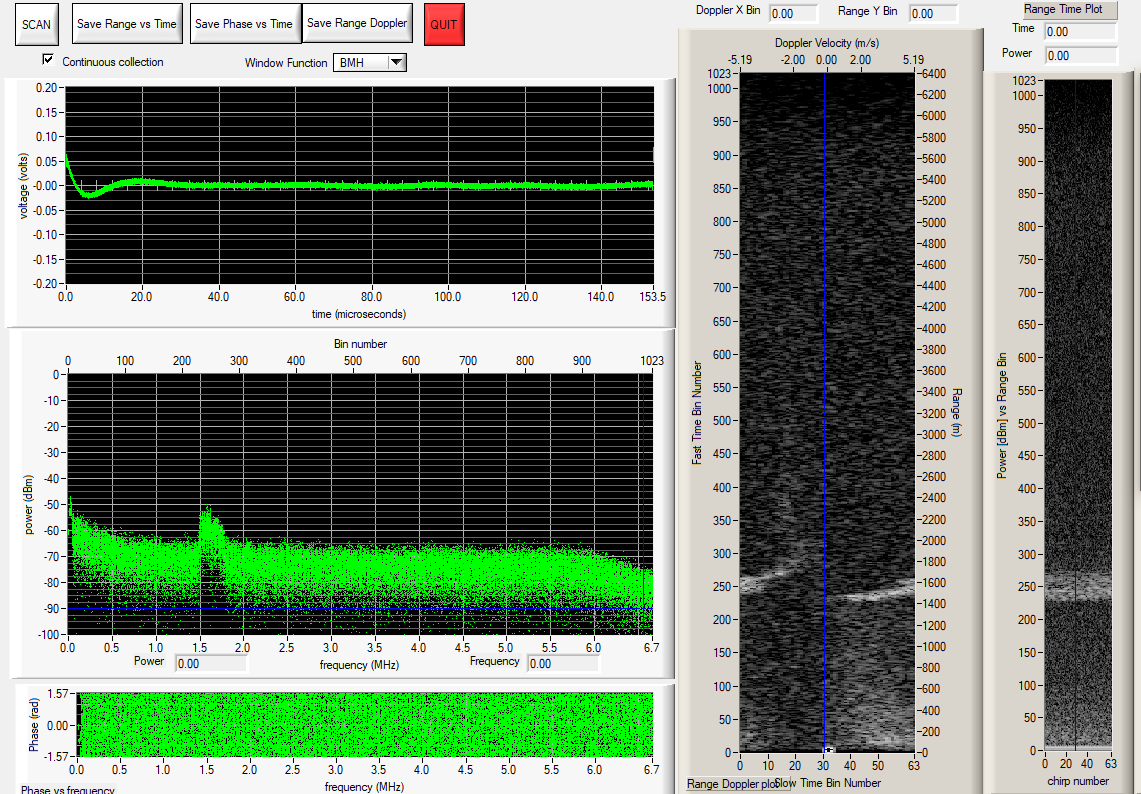
\includegraphics[width=\textwidth]{mark-1-rain}
	\caption{Screenshot of Mark I user interface, taken during precipitation.}
	\label{fig:Mark1Rain}
\end{figure}

\section{Design and implementation}
\begin{figure}
	\centering
	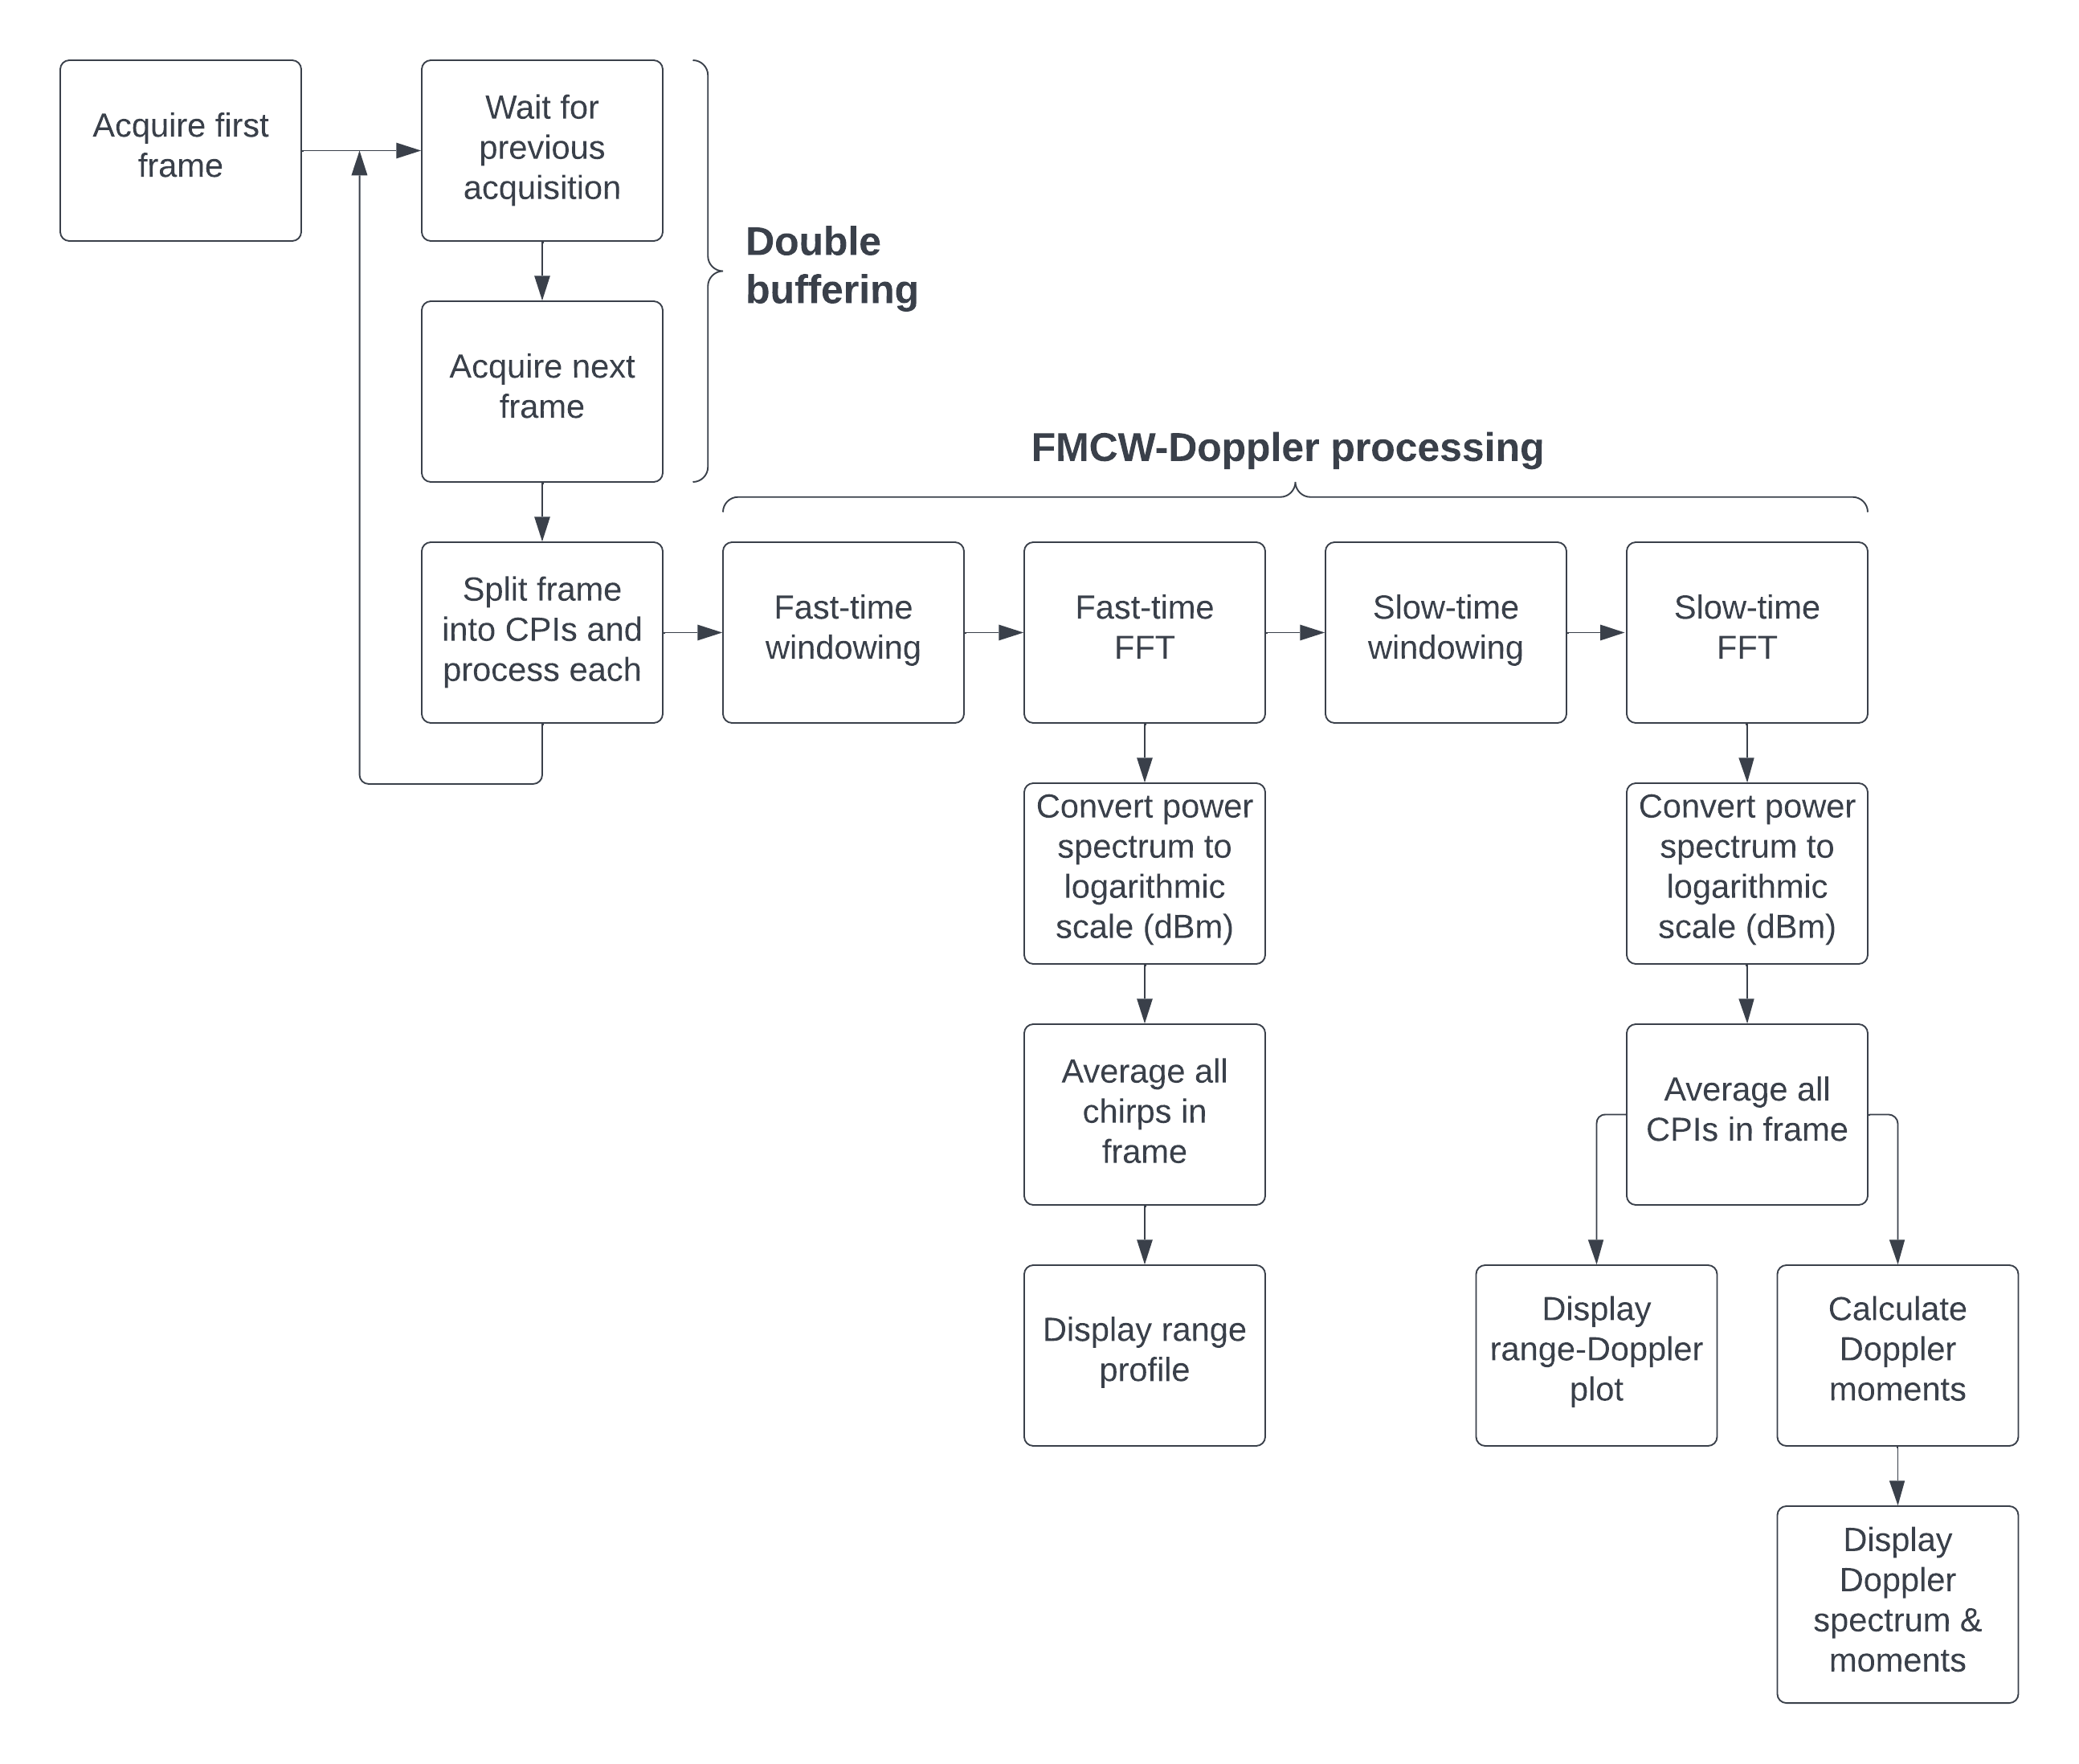
\includegraphics[width=\textwidth]{signal-processing-diagram}
	\caption{Simplified block diagram illustrating key signal processing steps. (Own work)}
	\label{fig:SignalProcessingDiagram}
\end{figure}

\subsection{Data acquisition}
\subsubsection{Double buffering}
To ensure real-time output, a double buffering approach is used.
One buffer is used to store the incoming frame and another stores the most recently acquired frame.
While the next frame is being acquired, the most recent frame is processed and displayed. The algorithm is shown in Alg. \ref{alg:DoubleBuffering}. Double buffering guarantees continuous real-time acquisition only if the processing time is less than the acquisition time.

\begin{algorithm}
	\centering
	\begin{algorithmic}
		\State acquire frame asynchronously into buffer $A$
		\While {keep acquiring data}
		\State wait for previous acquisition to finish
		\State acquire frame asynchronously into buffer $B$
		\State process frame in buffer $A$
		\State display processed frame
		\State swap $A$ and $B$ pointers
		\EndWhile
	\end{algorithmic}
	\caption{Double buffering approach.}\label{alg:DoubleBuffering}
\end{algorithm}

\subsubsection{Alternatives to double buffering}\label{sc:AltToDblBuf}
The approach in Mark II used one acquisition thread and one processing thread. The acquisition thread repeatedly acquires and appends frames to a thread-safe queue, which the processing thread pulls from.

The main issue with this approach is the acquisition thread wastes \acrshort{ac:cpu} time waiting for the frame to be acquired and transferred to memory.

\begin{algorithm}
	\begin{minipage}{0.48\linewidth}
		\begin{algorithmic}
			\While {keep acquiring data}
			\State acquire frame into buffer
			\State wait for previous acquisition to finish
			\State copy into thread safe queue
			\EndWhile
		\end{algorithmic}
	\end{minipage}
	\begin{minipage}{0.48\linewidth}
		\begin{algorithmic}
			\While {keep acquiring data}
			\State copy next frame in thread-safe queue
			\State process frame
			\State display processed frame
			\EndWhile
		\end{algorithmic}
	\end{minipage}
	\caption{Acquisition (left) and processing (right) threads.}\label{alg:TwoThreads}
\end{algorithm}

The double buffering approach uses only two buffers, which avoids unnecessary copying of data between threads and the additional overhead of using a thread-safe queue.

\subsection{FMCW-Doppler processing}
The software uses a third-party library, \acrshort{ac:fftw} v3\cite{FFTWv3}, for the two discrete Fourier transform steps in the FMCW-Doppler process.

Newer versions of LabWindows \acrshort{ac:cvi} use \acrshort{ac:fftw} behind the scenes, however the interface is not as flexible. \acrshort{ac:fftw} supports multiple transforms of non-unit stride,\footnote{Stride is the number of memory locations between each successive element in an array.} allowing one to easily perform multiple transforms along different dimensions. This is particularly useful for the column-wise slow-time transform, because it means the data does not need to be transposed before transforming. In \acrshort{ac:cvi}, the \acrshort{ac:fft} routines are limited to a single contiguous 1D array at a time. 

In \acrshort{ac:fftw}, \textit{plans} are created 

The window functions available in the new software are flat-top, Hann, Blackman, and Blackman-Harris.

\subsubsection{Averaging}
In each frame, two averaging processes take place. Averaging of power spectra is done over each chirp. For a frame containing \(256\) \acrshort{ac:cpi}s each containing \(64\) chirps, this amounts to \(16384\) chirps averaged together. 

\subsection{Testing}
To facilitate testing the software, a mock implementation of the \acrshort{ac:daq} was created. Raw data (\acrshort{ac:adc} integers) saved by the Mark II can be loaded by the mock implementation and used as if the data was just acquired. This feature is extremely useful for reproducible debugging and testing. A few snapshots of rain data were saved and used to test the new code when the weather was too clear.

A signal generator was attached to the second input channel of the \acrshort{ac:daq} card. Checking to see if the input power matches the peak value in the fast-time power spectrum provides confirmation that any corrections or scaling performed during the fast-time processing is correct.

Setting the input frequency to be slightly off bin centre introduces spectral leakage (Fig. \ref{fig:WindowNone}) Fig. \ref{fig:WindowBMH} shows the effect of applying the Blackman-Harris window is as expected.

\begin{figure}
	\centering
	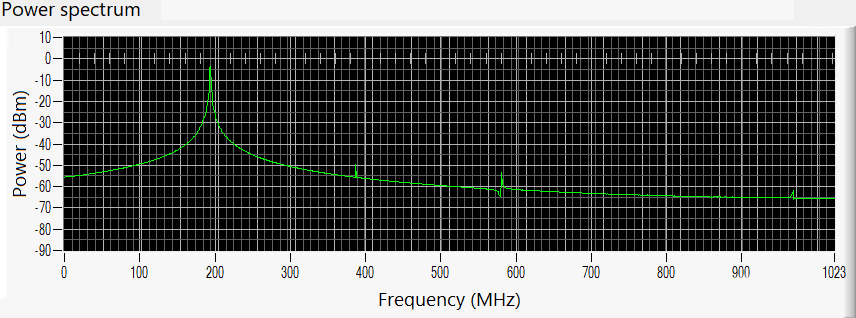
\includegraphics[width=\textwidth]{window-none}
	\caption{Fast-time power spectrum without windowing.}
	\label{fig:WindowNone}
\end{figure}

\begin{figure}
	\centering
	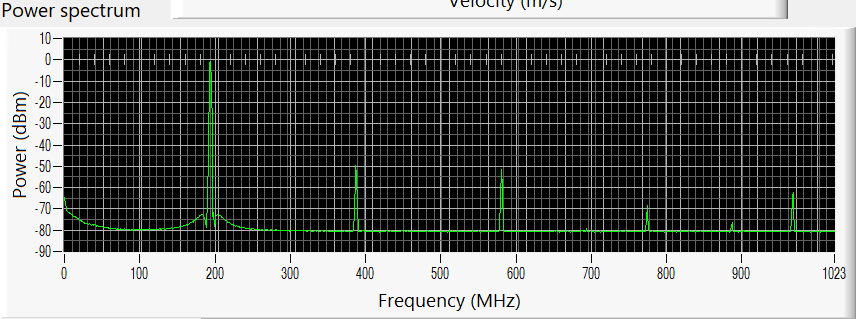
\includegraphics[width=\textwidth]{window-bmh}
	\caption{Fast-time power spectrum with Blackman-Harris windowing.}
	\label{fig:WindowBMH}
\end{figure}

\subsection{Averaging}
How is averaging implemented? Not much to say here really

\section{Results}

\begin{figure}
	\centering
	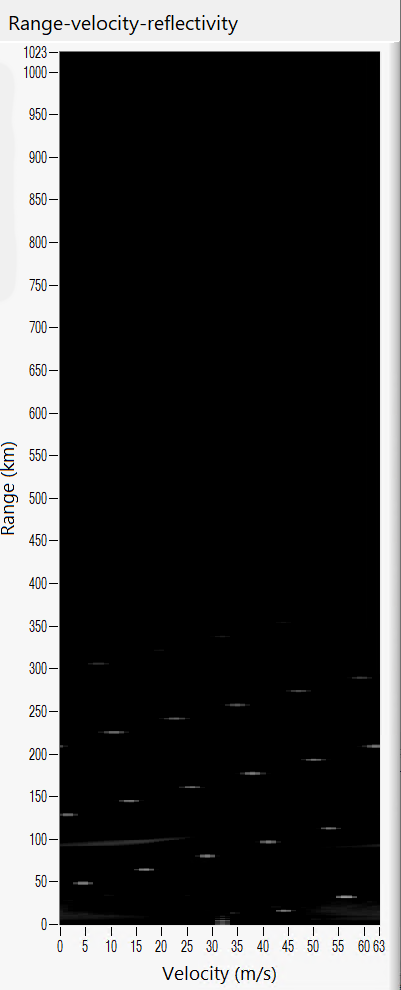
\includegraphics[width=0.4\textwidth]{working-cloud_range-doppler}
	\caption{Screenshot of the new user interface.}
	\label{fig:WorkingCloudRangeDoppler}
\end{figure}

\begin{figure}
	\centering
	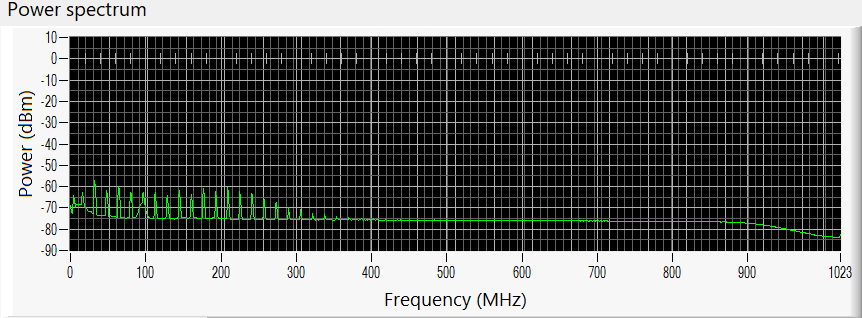
\includegraphics[width=\textwidth]{working-cloud_power-spect}
	\caption{Screenshot of the new user interface.}
	\label{fig:WorkingCloudPowerSpectrum}
\end{figure}

\begin{figure}
	\centering
	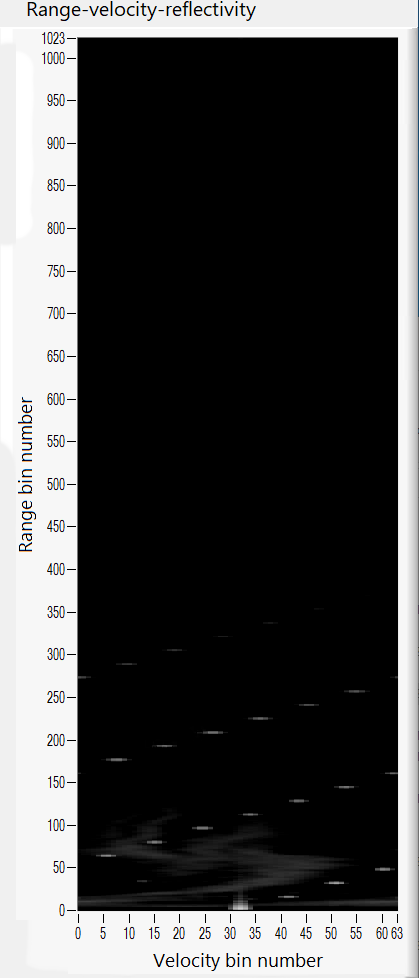
\includegraphics[width=0.4\textwidth]{working-hail_range-doppler}
	\caption{Screenshot of the new user interface.}
	\label{fig:WorkingHailRangeDoppler}
\end{figure}

\begin{figure}
	\centering
	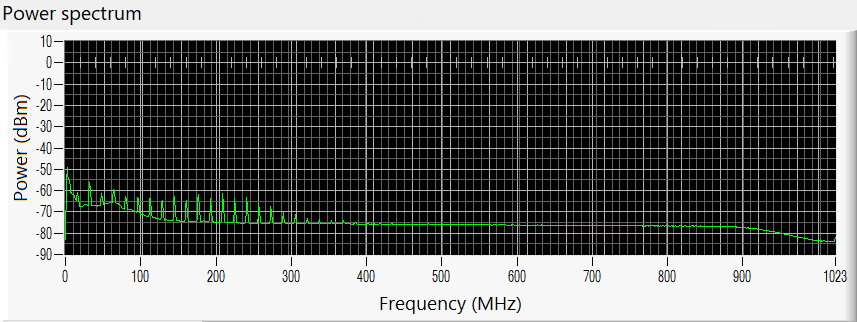
\includegraphics[width=\textwidth]{working-hail_power-spect}
	\caption{Screenshot of the new user interface.}
	\label{fig:WorkingHailPowerSpectrum}
\end{figure}

\begin{figure}
	\centering
	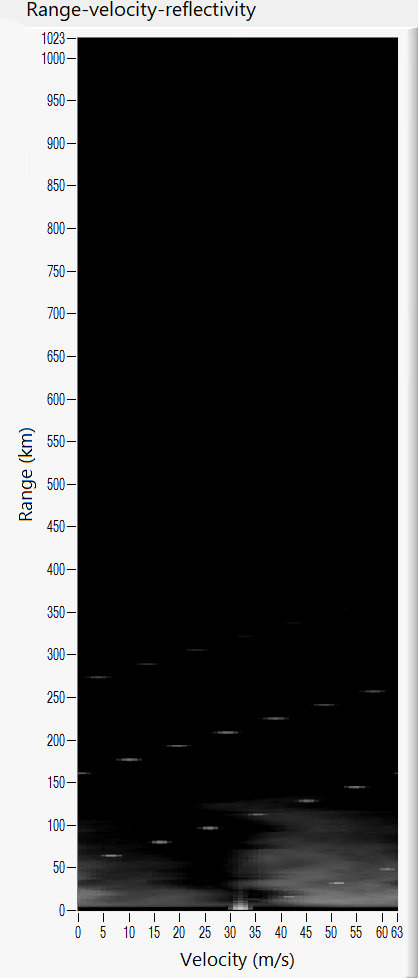
\includegraphics[width=0.4\textwidth]{working-heavy-rain-sleet_range-doppler}
	\caption{Screenshot of the new user interface.}
	\label{fig:WorkingHeavyRainSnowRangeDoppler}
\end{figure}

\begin{figure}
	\centering
	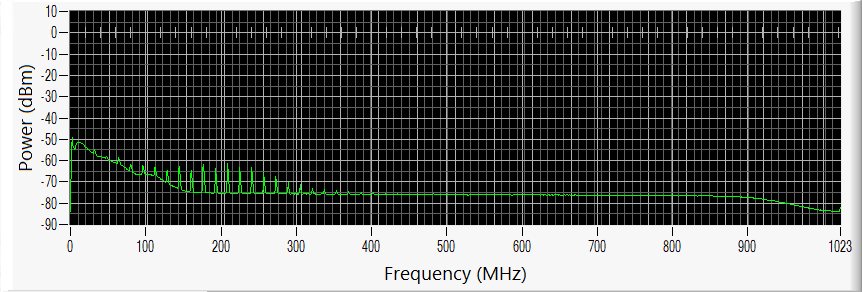
\includegraphics[width=\textwidth]{working-heavy-rain-sleet_power-spect}
	\caption{Screenshot of the new user interface.}
	\label{fig:WorkingHeavyRainSnowPowerSpectrum}
\end{figure}

\subsection{Performance}
The results in Tbl. \ref{tbl:ProcTime} show that the new code has continuous, real time acquisition. One \acrshort{ac:cpi} containing \(64\) chirps each with \(2048\) samples lasts for \(\SI{19.7}{\milli\second}\), which is more than the processing time of \(\SI{13.9(1)}{\milli\second}\).

\begin{table}[H]
	\centering
	\begin{tabular}{|c|c|}
		\hline
		        & Processing time             \\
		\hline
		Mark II & \SI{67.6(6)}{\milli\second} \\
		\hline
		New     & \SI{13.9(1)}{\milli\second} \\
		\hline
	\end{tabular}
	\caption{Processing time of Mark II vs new code. Measured as the time taken to process one \acrshort{ac:cpi} (\(64\) chirps, \(2048\) samples). For new code this also includes power spectrum averaging and Doppler moment extraction. Number of samples: \(400\). Both built using \acrshort{ac:cvi} v19.0.0. Release build.}
	\label{tbl:ProcTime}
\end{table}

There are several reasons for the speed improvements in the new code.
Both the Mark I and Mark II frequently copy data into temporary arrays while processing, which is avoided in the new code.
In addition, these temporary arrays are variable-length (\acrshort{ac:vla}s) which are generally slower than arrays with a size known at compile-time or dynamically allocated arrays.
The new code leverages \acrshort{ac:fftw}'s advanced interface to \acrshort{ac:fft} the entire 2D \acrshort{ac:cpi} array in one go. Since \acrshort{ac:fftw} knows the dimensions of the input it might be using optimisations suited for multidimensional transforms.

\section{Future work}
\subsection{Calibration}
Currently the output power is in \(\si{\deci\belm}\) rather than \(\si{\deci\belz}\). Since the conversion to \(\si{\deci\belz}\) is dependent on bandwidth and the hardware control was not fully implemented, it was decided to not convert to \(\si{\deci\belz}\) yet.

\subsection{Doppler moments}
Extracting the Doppler spectrum from the averaged range-Doppler data has already been implemented along with UI controls for displaying Doppler moments, however the results are wildly incorrect. 

the formulas used for determining the moments are incorrect.

\subsection{Effect of ambient temperature}
\subsection{NetCDF}

\subsection{Performance improvements}
\subsubsection{Multithreading}
Many of the calculations in the \acrshort{ac:fmcw}-Doppler process are highly parallel and are performed on large 

An easy way of parallelising loops with is to use \acrshort{ac:openmp}

\subsubsection{SIMD}
Single instruction, multiple data (\acrshort{ac:simd}) is another type of parallel processing where a single instruction operates simultaneously on multiple pieces of data. \acrshort{ac:fftw} uses this extensively. Many of the steps in the \acrshort{ac:fmcw}-Doppler process are adding or multiplying rows or columns by the same constants which makes \acrshort{ac:simd} highly effective.

\section{Conclusions}

\clearpage
\printbibliography

\end{document}
